\documentclass{beamer}

\usepackage{graphicx}
\usepackage{color}
\usepackage{listings}

\usetheme{Boadilla}

\AtBeginSection[]{
    \begin{frame}
    \vfill
    \centering
      \usebeamerfont{title}\insertsectionhead\par%
    \vfill
    \end{frame}
}

\definecolor{darkgreen}{rgb}{0,0.6,0}
\definecolor{darkorange}{rgb}{1,0.4,0}

\lstdefinestyle{codestyle}{
    backgroundcolor=\color{white},
    commentstyle=\color{darkgreen},
    keywordstyle=\color{blue},
    numberstyle=\color{black},
    stringstyle=\color{darkorange},
    basicstyle=\ttfamily\footnotesize,
    breakatwhitespace=false,
    breaklines=true,
    captionpos=b,
    keepspaces=true,
    numbers=none,
    showspaces=false,
    showstringspaces=false,
    showtabs=false,
    breaklines=true,
}

\lstset{style=codestyle}

\title{Esplorare L'API Grafica Vulkan}
\author{Emanuele Franchi}
\date{}

\begin{document}

\begin{frame}

\titlepage

\end{frame}


\begin{frame}
\frametitle{Vulkan}

\begin{itemize}
\item API grafica sotto forma di specifica
\item Non ne esiste un'unica implementazione
\item Implementata attraverso il driver della propria scheda grafica
\item Sviluppata usando come modello l'architettura delle GPU odierne
\item API di basso livello
\item Richiede un certo know how da parte del programmatore
\item Se il programmatore la utilizza in modo coscienzioso, può risultare in performance migliori rispetto alle API di vecchia generazione
\item Multithreaded first
\end{itemize}

\end{frame}

\begin{frame}
\frametitle{Inizializzare Vulkan}

\begin{itemize}
\item Creiamo una Vulkan instance
\item Creiamo una finestra (OS)
\item Creiamo una presentation surface
\item Selezioniamo una GPU (device fisico)
\item Creiamo un device logico per interfacciarsi con la GPU
\item Creiamo una swapchain per gestire la presentazione d'immagini sulla presentation surface
\end{itemize}

\end{frame}

\begin{frame}
\frametitle{Renderizzare Un Colore: Demo}
\begin{figure}[ht]
    \centering
    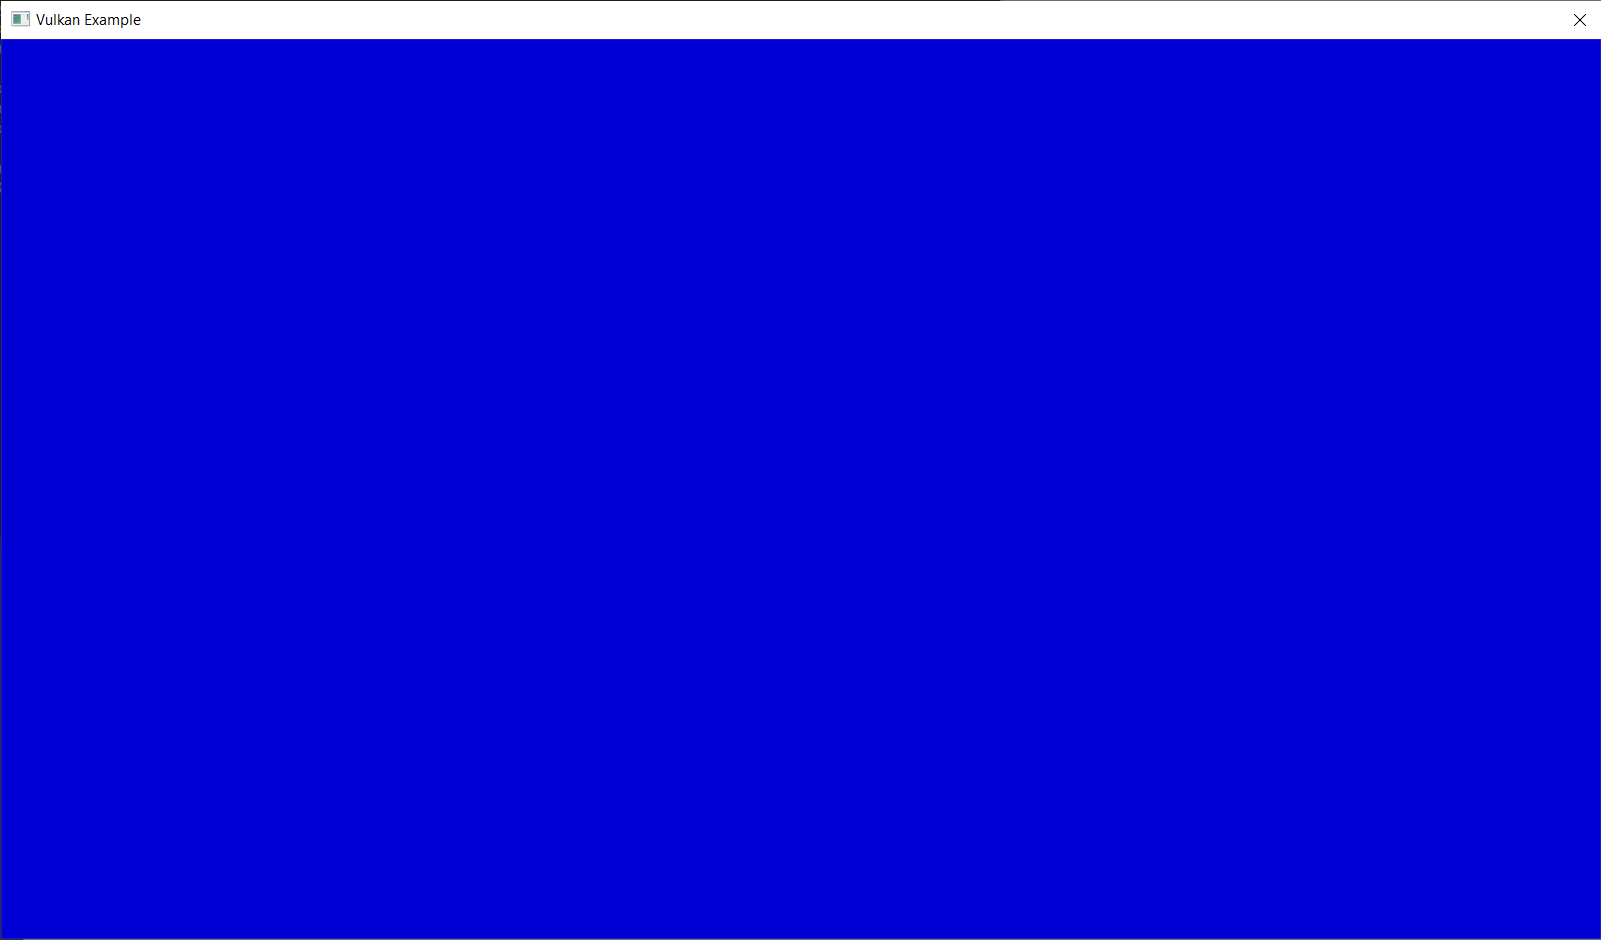
\includegraphics[scale=0.25]{images/SlidesClearWindow/ClearWindow.png}
\end{figure}
\end{frame}

\begin{frame}
\frametitle{Renderizzare Un Colore}

\begin{itemize}
\item Creiamo un render pass
\item Un render pass descrive gli attachment che vengono utilizzati durante il rendering
\item Un render pass raggruppa i comandi grafici in uno o più subpass in base a come e quali attachment utilizzano
\item Creiamo un framebuffer
\item Un reamebuffer è l'insieme di attachment utilizzati da un'istanza di un render pass
\item Creiamo un command buffer
\item Scriviamo comandi sul command buffer
\item Inviamo il command buffer alla GPU
\item Presentiamo un'immagine della swapchain sulla presentation surface
\end{itemize}
\end{frame}

\begin{frame}
\frametitle{Renderizzare Un Triangolo: Demo}
\begin{figure}[ht]
    \centering
    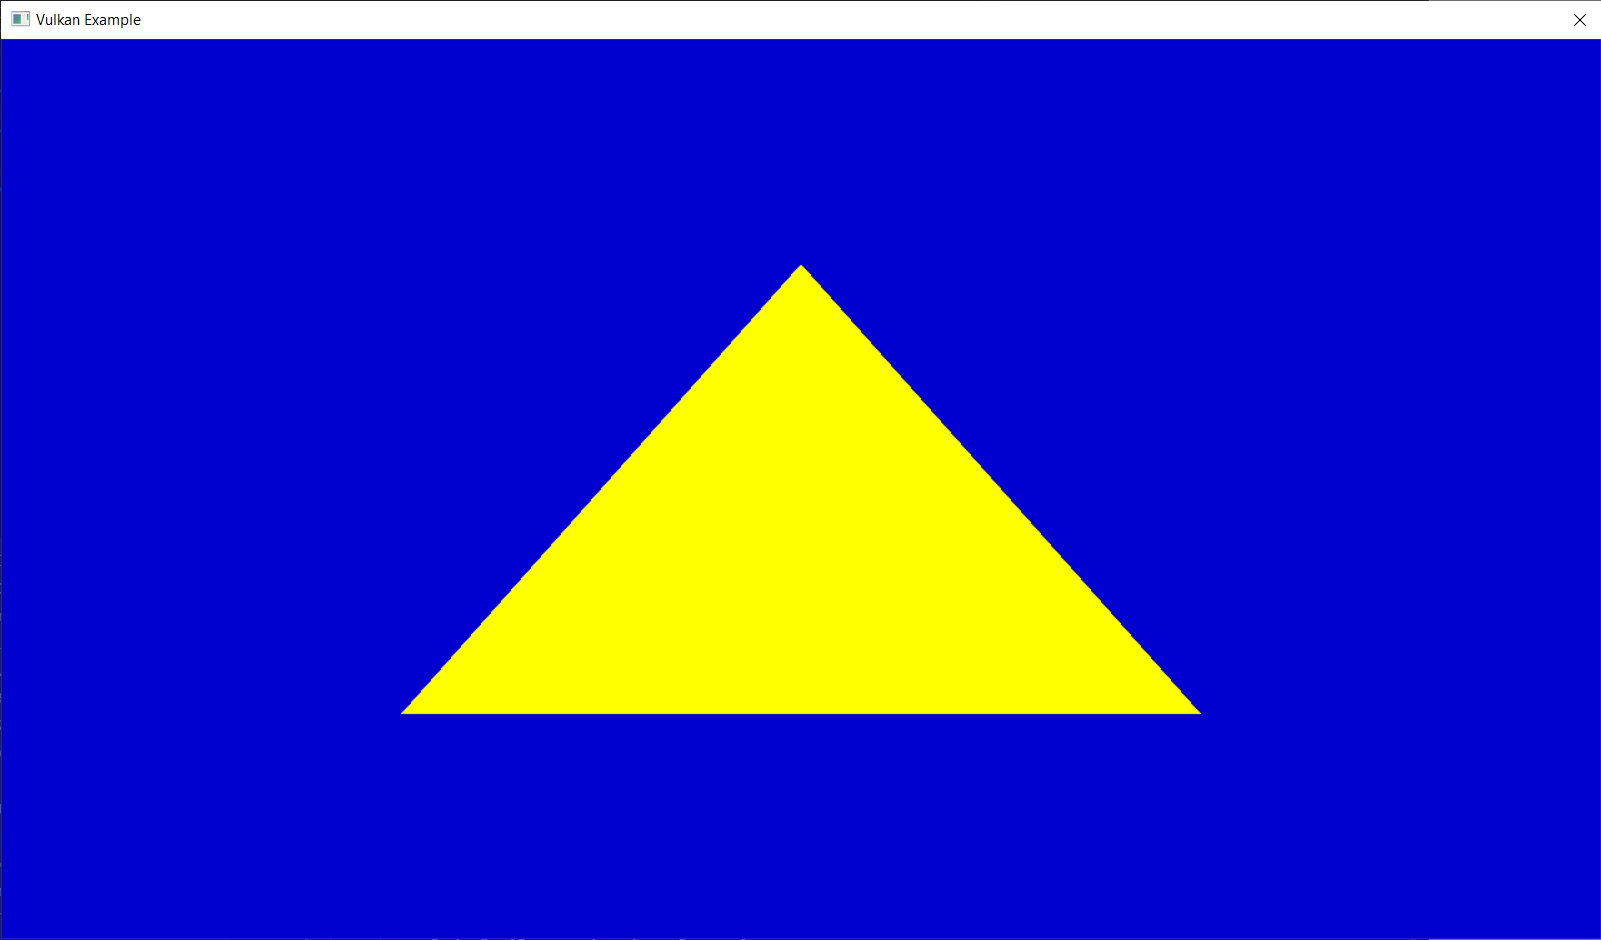
\includegraphics[scale=0.25]{images/SlidesTriangle/Triangle.png}
\end{figure}
\end{frame}

\begin{frame}
\frametitle{Renderizzare Un Triangolo}
\begin{itemize}
\item Creiamo un pipeline state object
\item Un pipeline state object descrive l'intero stato della pipeline grafica
\item Shader: programmi eseguiti dalla GPU
\item In particolare vertex shader e un fragment shader
\item La pipeline grafica riceve come input una sequenza di vertici
\item La pipeline grafica esegue il vertex shader per ogni vertice
\item Il vertex shader genera della geometria
\item La pipeline grafica esegue il fragment shader per ogni pixel coperto dalla geometria
\end{itemize}
\end{frame}

\begin{frame}
\frametitle{Vertici: Demo}
\begin{figure}[ht]
    \centering
    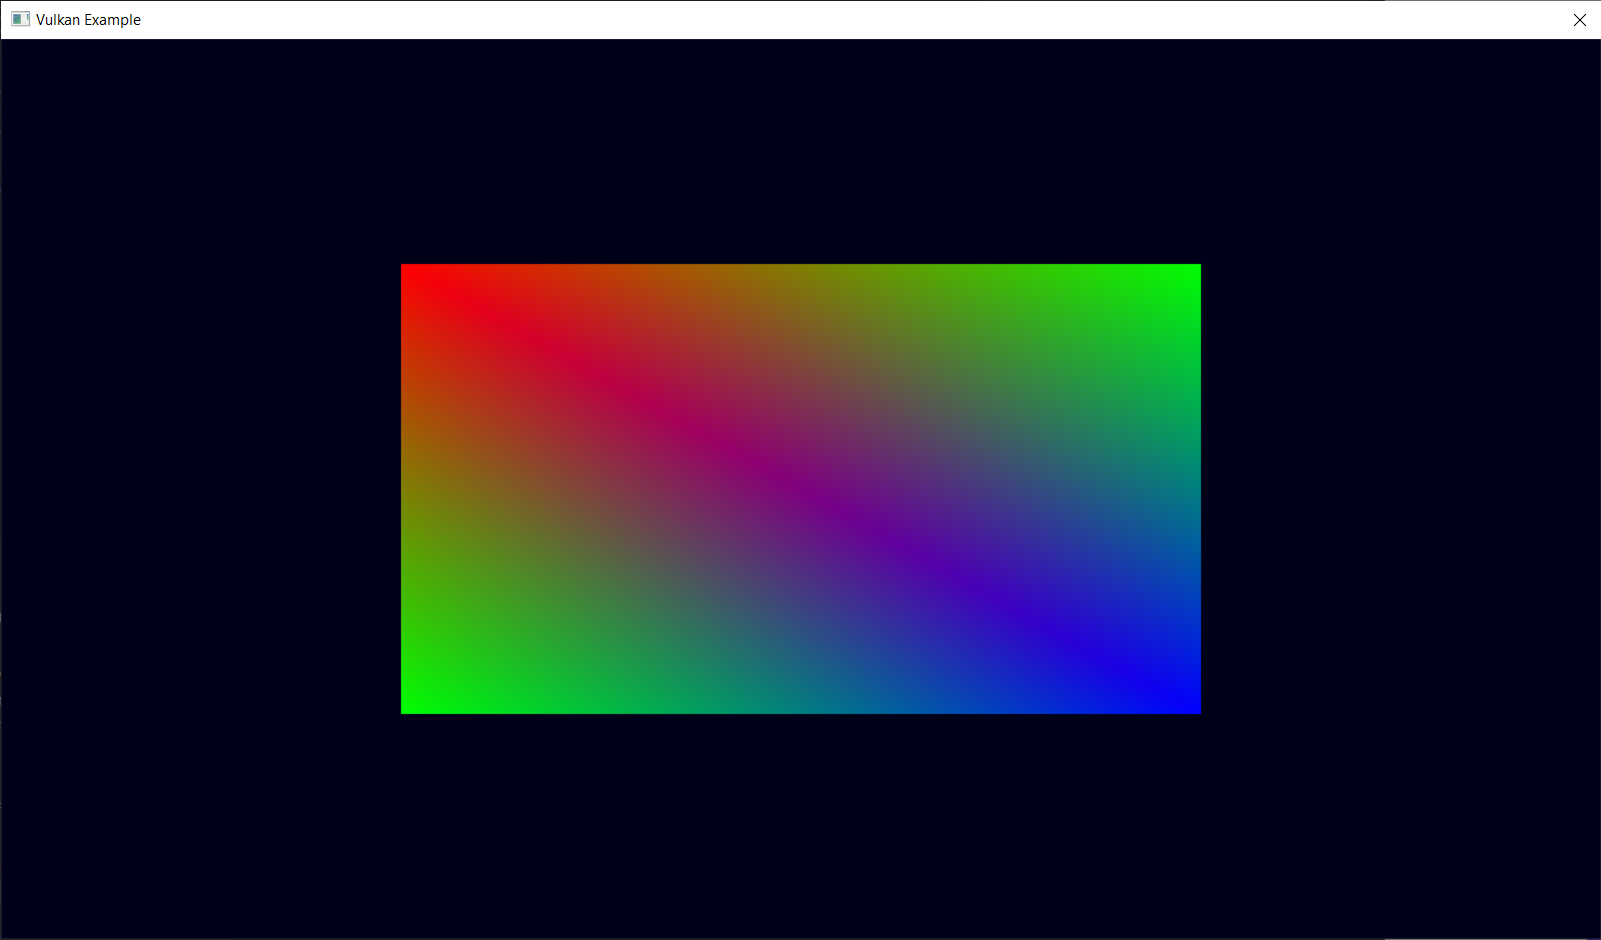
\includegraphics[scale=0.25]{images/SlidesVertices/RenderQuad.png}
\end{figure}
\end{frame}

\begin{frame}
\frametitle{Vertici}
\begin{itemize}
\item I dati dei nostri vertici sono in RAM e noi dobbiamo caricarli nella memoria della GPU
\item Usiamo due buffer
\item Uno staging buffer, allocato su memoria della GPU host visible
\item Scriviamo i dati dei nostri vertici su questo buffer
\item Un vertex buffer, allocato su memoria della GPU device local
\item Inviamo un comando che dice alla GPU di trasferire il contenuto dello staging buffer nel vertex buffer
\item Modifichiamo la creazione del nostro pipeline state object per specificare come interpretare i dati nel vertex buffer
\item Prima di registrare il comando per attivare la pipeline, registriamo un comando che indica alla pipeline grafica di usare come input il nostro vertex buffer
\end{itemize}
\end{frame}

\begin{frame}
\frametitle{Uniform Buffer: Demo}
\begin{figure}[ht]
    \centering
    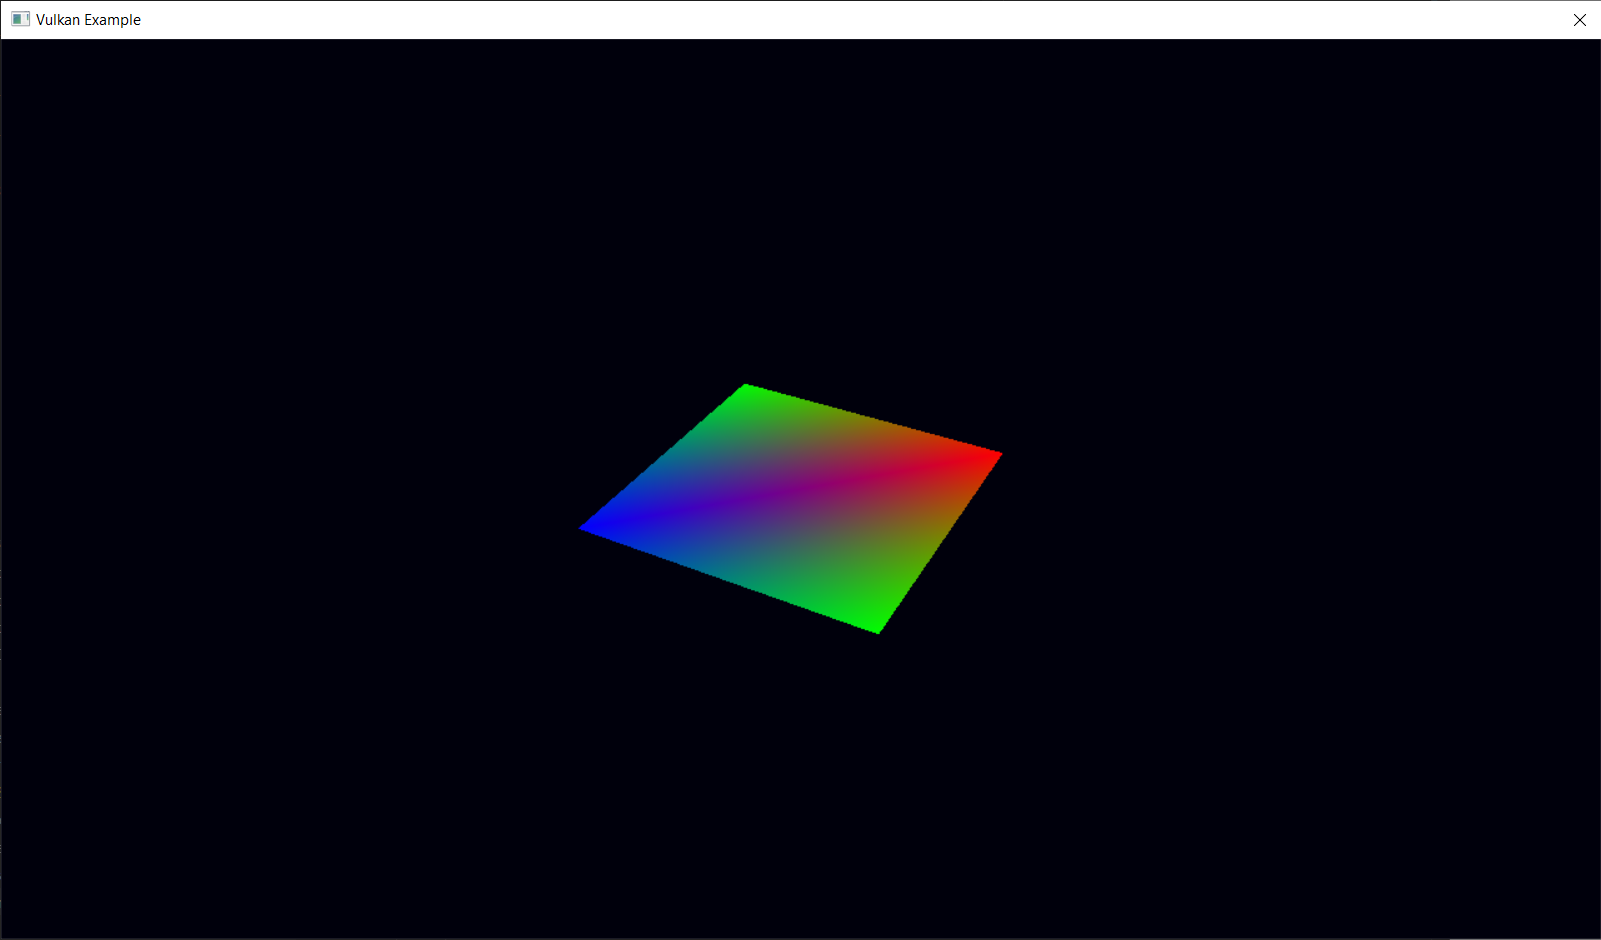
\includegraphics[scale=0.25]{images/SlidesUniforms/RenderQuad.png}
\end{figure}
\end{frame}

\begin{frame}
\frametitle{Uniform Buffer}
\begin{itemize}
\item Una variabile globale di uno shader è detta uniform
\item Passiamo le variabili globali agli shader usando uno uniform buffer
\item Siccome tali variabili cambiano frequentemente, allochiamo uno uniform buffer su memoria della GPU host visible
\item Creiamo un pipeline layout object
\item Un pipeline layout object descrive quali descriptor sono accessibili in quali shader
\item Creiamo un descriptor set layout
\item Un descriptor set layout descrive il contenuto di un descriptor set
\item Creiamo un descriptor set basandoci sul descriptor set layout
\item Una volta allocato, un descriptor set va popolato con i descriptor appropriati
\end{itemize}
\end{frame}

\begin{frame}
\frametitle{Depth Buffer: Demo}

\begin{columns}

\column{.5\textwidth}

\begin{figure}[ht]
    \centering
    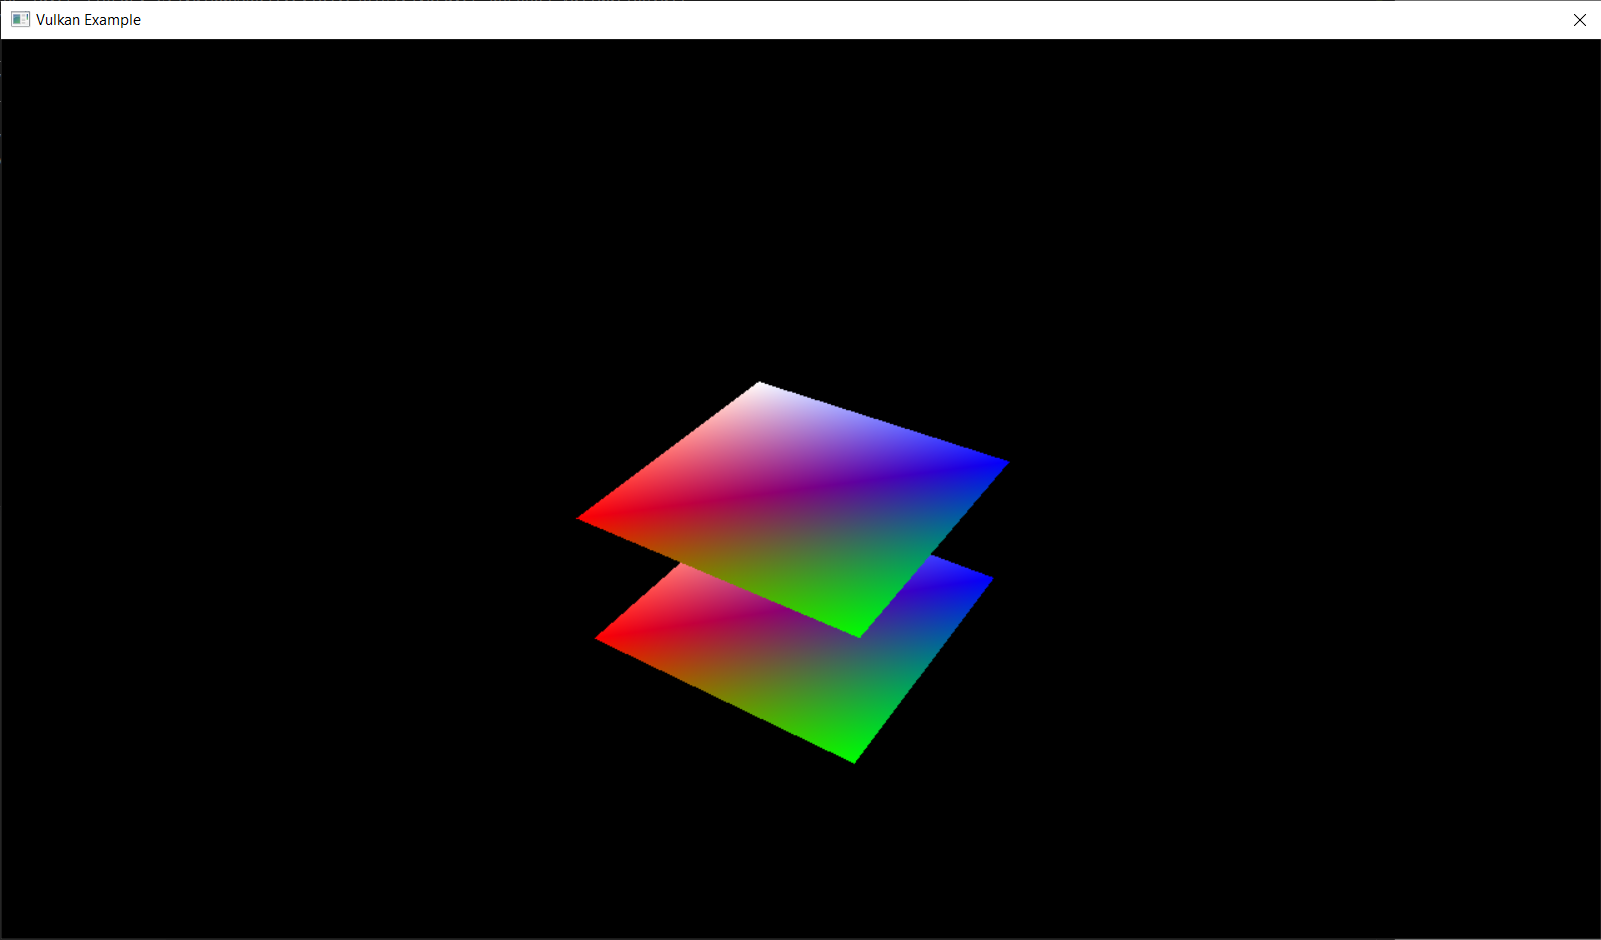
\includegraphics[scale=0.14]{images/SlidesDepthTesting/DepthTesting.png}
\end{figure}

\column{.5\textwidth}

\begin{figure}[ht]
    \centering
    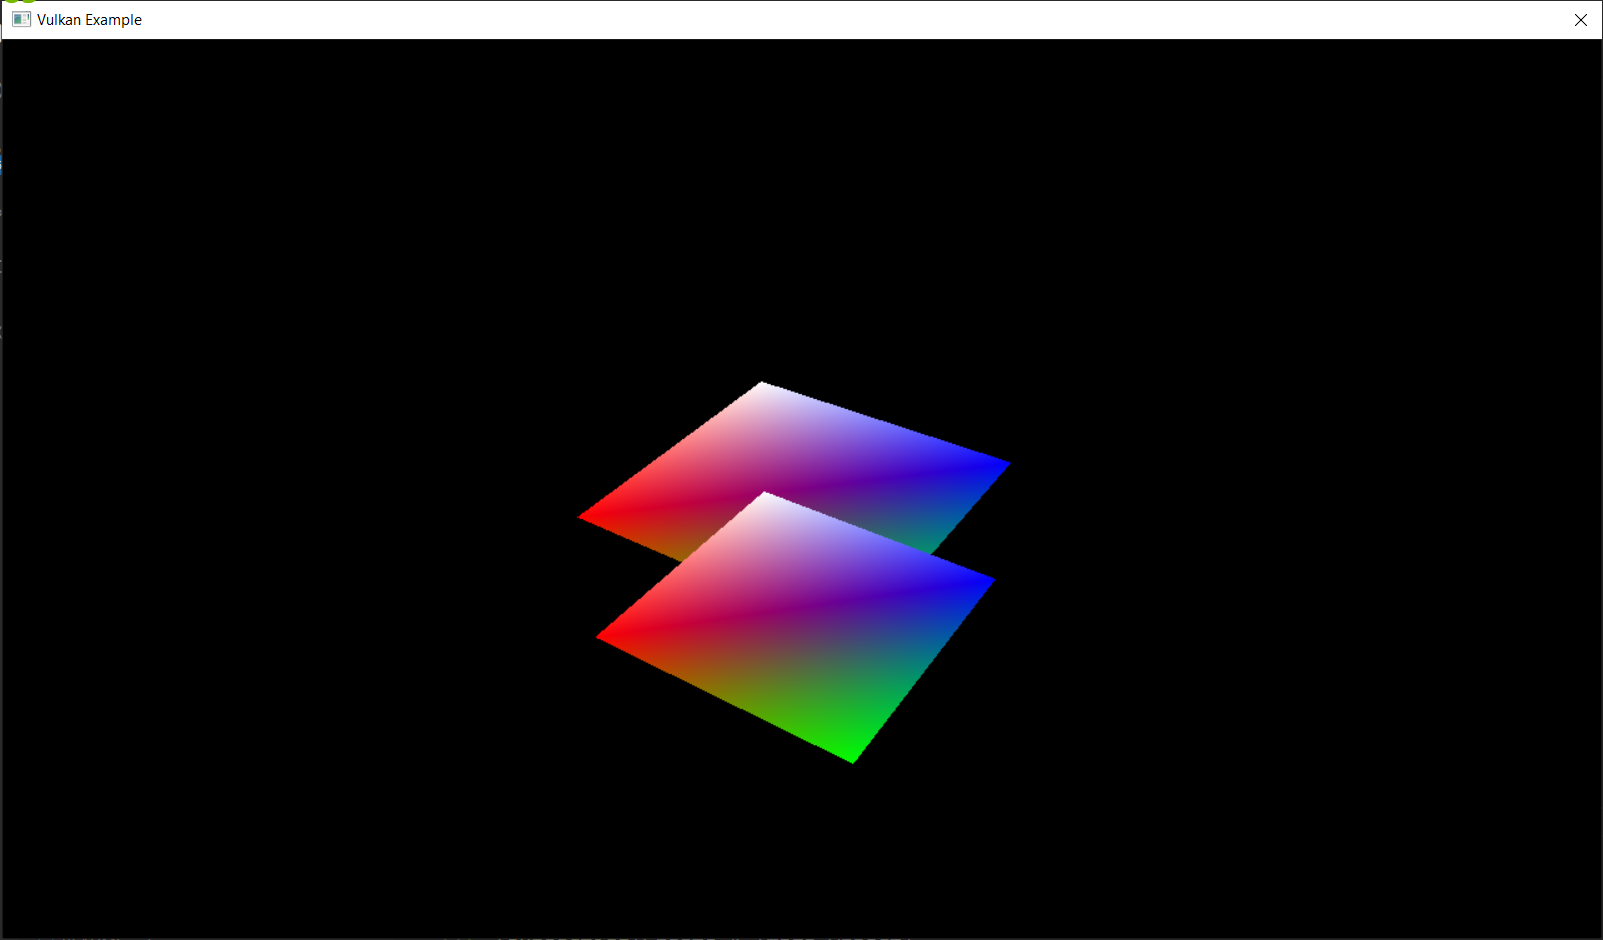
\includegraphics[scale=0.14]{images/SlidesDepthTesting/NoDepthTesting.png}
\end{figure}

\end{columns}

\end{frame}

\begin{frame}
\frametitle{Depth Buffer}
\begin{itemize}
\item Come renderizzare oggetti in modo tale che quelli più vicini possano nascondere quelli più lontani?
\item Possiamo ordinare gli oggetti in base alla loro lontananza dalla camera
\item E se due oggetti si sovrappongono?
\item Se gli oggetti da renderizzare sono opachi, usiamo un depth buffer
\item Un depth buffer è un'immagine che codifica informazioni riguardanti la profondità dei frammenti
\item Quando un frammento viene generato, compariamo la sua profondità con quella salvata nel corrispettivo texel del depth buffer
\item Se è più grande, il frammento non viene ignorato
\item Se è più piccola, il frammento viene utilizzato e la sua profondità viene salvata nel depth buffer
\item Creiamo un'immagine da usare come depth stencil attachment
\item Abilitiamo il depth testing quando creiamo il pipeline state object
\end{itemize}
\end{frame}

\begin{frame}
\frametitle{Scene}
\begin{columns}


\column{.6\textwidth}


\begin{itemize}
\item
\end{itemize}


\column{.2\textwidth}


\end{columns}
\end{frame}

\begin{frame}
\frametitle{Blinn-Phong: Demo}
\begin{figure}[ht]
    \centering
    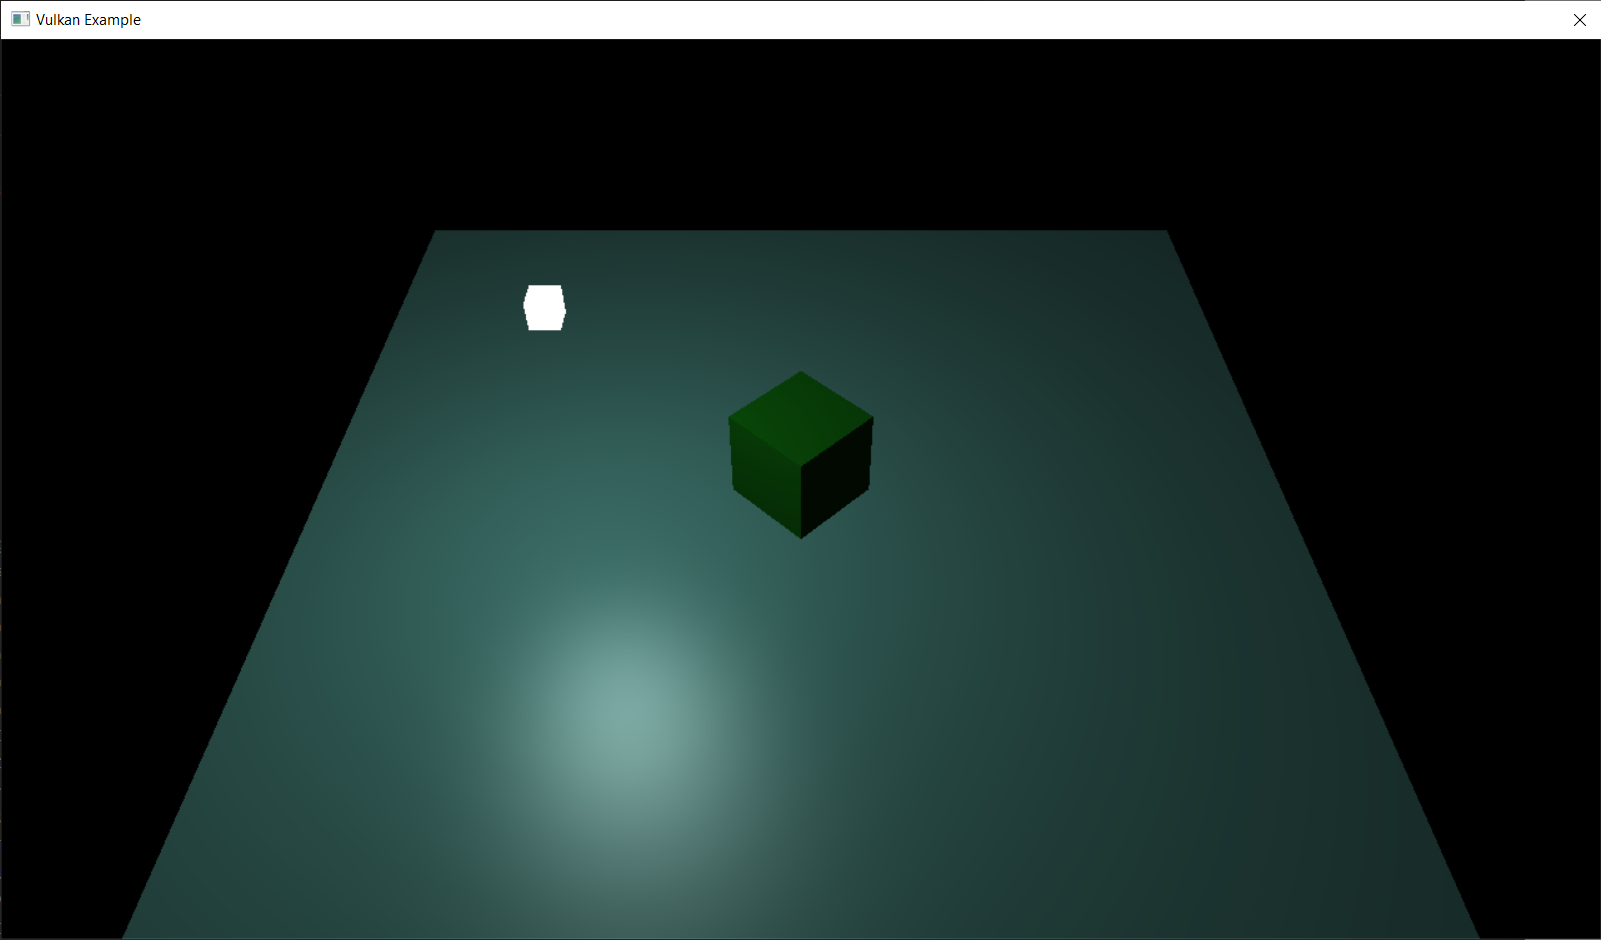
\includegraphics[scale=0.25]{images/SlidesBlinnPhong/SceneMaterialsLight.png}
\end{figure}
\end{frame}

\begin{frame}
\frametitle{Blinn-Phong}
\begin{itemize}
\item L'illuminazione viene divisa in tre componenti: ambient, diffuse e specular
\item La componente ambientale modella il fatto che una scena non è mai totalmente buia
\item La componente diffusiva simula l'impatto che la luce ha sugli oggetti opachi
\item La componente speculare simula il punto luminoso che una luce causa su oggetti lucidi (specular highlight)
\item Ogni oggetto ha un materiale: componente ambientale, diffusiva, speculare e lucentezza
\item Una luce ha diverse intensità per la componente ambientale, diffusiva e speculare
\end{itemize}
\end{frame}

\begin{frame}
\frametitle{MSAA: Demo}
\begin{figure}[ht]
    \centering
    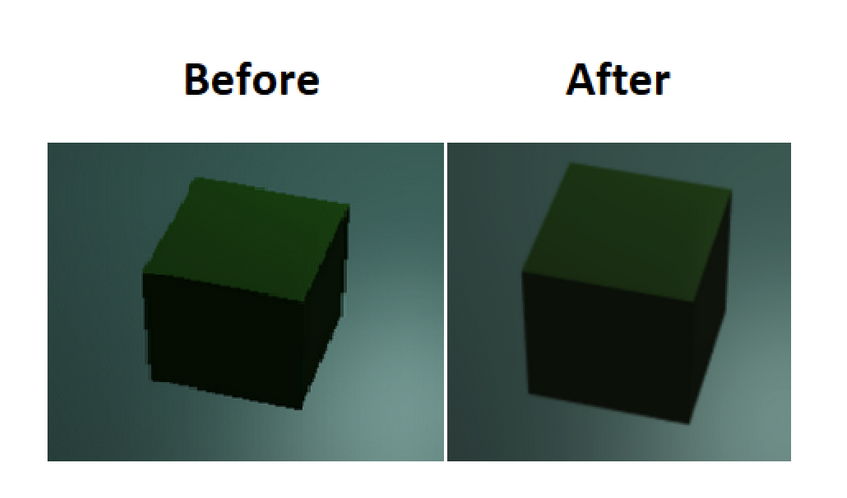
\includegraphics[scale=0.50]{images/SlidesMSAA/BeforeAfterMSAA.png}
\end{figure}
\end{frame}

\begin{frame}
\frametitle{MSAA: Un Campione Per Pixel}
\begin{figure}[ht]
    \centering
    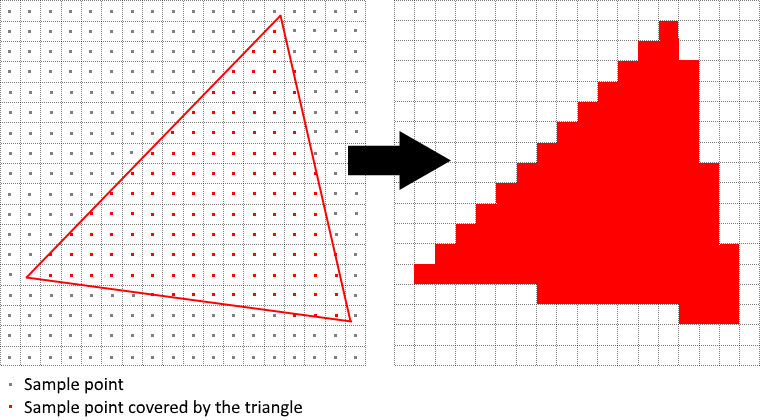
\includegraphics[scale=0.50]{images/SlidesMSAA/OneSamplePerPixel.png}
\end{figure}
\end{frame}

\begin{frame}
\frametitle{MSAA: Quattro Campioni Per Pixel}
\begin{figure}[ht]
    \centering
    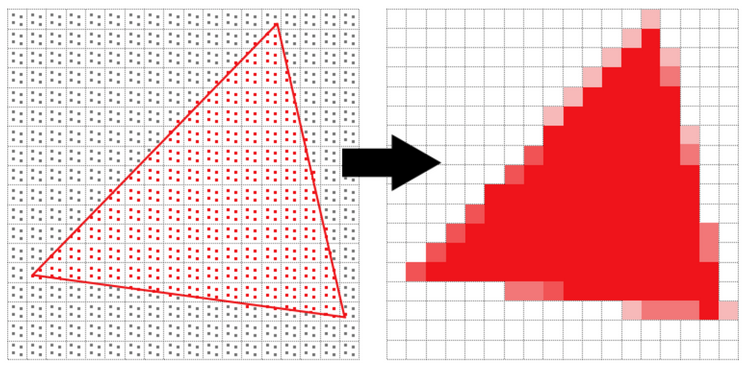
\includegraphics[scale=0.50]{images/SlidesMSAA/FourSamplesPerPixel.png}
\end{figure}
\end{frame}

\begin{frame}
\frametitle{MSAA}
\begin{itemize}
\item Le immagini che supportano il multisampling non sono presentabili
\item Tutte le immagini presentabili devono avere un solo campione per pixel
\item Creiamo una nuova immagine che abbia il numero di campioni per pixel che desideriamo
\item Useremo questa immagine come nuovo color attachment nel render pass
\item Usiamo l'immagine della swapchain come color resolve attachment
\item Non dobbiamo dimenticarci di abilitare l'uso del multisampling quando creiamo un pipeline state object
\end{itemize}
\end{frame}


\end{document}
